\let\negmedspace\undefined
\let\negthickspace\undefined
\documentclass[journal]{IEEEtran}
\usepackage[a5paper, margin=10mm, onecolumn]{geometry}
%\usepackage{lmodern} % Ensure lmodern is loaded for pdflatex
\usepackage{tfrupee} % Include tfrupee package

\setlength{\headheight}{1cm} % Set the height of the header box
\setlength{\headsep}{0mm}     % Set the distance between the header box and the top of the text
\usepackage{gvv-book}
\usepackage{gvv}
\usepackage{cite}
\usepackage{amsmath,amssymb,amsfonts,amsthm}
\usepackage{algorithmic}
\usepackage{graphicx}
\usepackage{textcomp}
\usepackage{xcolor}
\usepackage{txfonts}
\usepackage{listings}
\usepackage{enumitem}
\usepackage{mathtools}
\usepackage{gensymb}
\usepackage{comment}
\usepackage[breaklinks=true]{hyperref}
\usepackage{tkz-euclide} 
\usepackage{listings}
% \usepackage{gvv}                                        
\def\inputGnumericTable{}                                 
\usepackage[latin1]{inputenc}                                
\usepackage{color}                                            
\usepackage{array}                                            
\usepackage{longtable}                                       
\usepackage{calc}                                             
\usepackage{multirow}                                         
\usepackage{hhline}                                           
\usepackage{ifthen}                                           
\usepackage{lscape}



\usepackage{amsmath,amssymb}
\usepackage{booktabs}
\usepackage{tikz}
\usetikzlibrary{arrows.meta,angles,quotes}





\begin{document}

\bibliographystyle{IEEEtran}
\vspace{3cm}

\title{1.2.29}
\author{AI25BTECH11021 - Abhiram Reddy N}
% \maketitle
% \newpage
% \bigskip
{\let\newpage\relax\maketitle}

\renewcommand{\thefigure}{\theenumi}
\renewcommand{\thetable}{\theenumi}
\setlength{\intextsep}{10pt} % Space between text and floats


\numberwithin{equation}{enumi}
\numberwithin{figure}{enumi}
\renewcommand{\thetable}{\theenumi}


\textbf{Question}:\\In a harbour, wind is blowing at the speed of $72\ \mathrm{km/h}$ and the flag on the mast of a boat anchored in the harbour flutters along the N--E direction. If the boat starts moving at a speed of $51\ \mathrm{km/h}$ to the north, what is the direction of the flag on the mast of the boat?


\textbf{Solution}:\\
Choose axes: $+\!y$ = North, $+\!x$ = East. \\
Wind vector (ground frame), pointing NE (45°):
\[
\mathbf{W}=72\big(\cos 45^\circ\,\mathbf{i}+\sin 45^\circ\,\mathbf{j}\big)
= \big(72/\sqrt2,\;72/\sqrt2\big).
\]
Boat velocity (ground frame) northward:
\[
\mathbf{V}=(0,\;51).
\]
Relative wind (wind seen from boat) is
\[
\mathbf{R}=\mathbf{W}-\mathbf{V}
=\Big(\tfrac{72}{\sqrt2},\;\tfrac{72}{\sqrt2}-51\Big).
\]
Numerically,
\[
\mathbf{R}\approx(50.9117,\; -0.08831)\ \mathrm{km/h}.
\]
Magnitude:
\[
\|\mathbf{R}\| \approx 50.9118\ \mathrm{km/h}.
\]
Direction: angle measured from the East axis (positive = north of east)
\[
\theta=\arctan\frac{y}{x}=\arctan\frac{-0.08831}{50.9117}\approx -0.0994^\circ.
\]
So the relative wind (flag) points \textbf{about $0.099^\circ$ south of east} (i.e. almost due east).



\begin{table}[h!]    
      \centering
      \begin{center}
    \begin{tabular}{|c|c|} 
        \hline
            \textbf{Variable}  & \textbf{Formula} \\ 
        \hline
            $a$   & $a = \myvec{4 \\ -1 \\ 1}$ \\ 
        \hline
            $b$   &  $b = \myvec{2 \\ -2 \\ 1}$\\ 
        \hline
           \end{tabular}
\end{center}  

      \caption{variables and numerical values}
    \end{table}


\begin{figure}[htbp]
\centering

\centering
\begin{tikzpicture}[>=Stealth,scale=0.9]
  % scaling factor (so vectors fit nicely)
  \def\sc{0.09}

  % numerical components
  \def\Wx{50.9117}
  \def\Wy{50.9117}
  \def\Vx{0}
  \def\Vy{51}
  \def\Rx{50.9117}
  \def\Ry{-0.0883}

  % --- Axes ---
  \draw[->] (-0.5,0) -- (7.5,0) node[right] {East ($+\mathbf{i}$)};
  \draw[->] (0,-1) -- (0,6.5) node[above] {North ($+\mathbf{j}$)};

  % origin
  \coordinate (O) at (0,0);

  % scaled coordinates
  \coordinate (W) at ({\sc*\Wx},{\sc*\Wy});
  \coordinate (V) at ({\sc*\Vx},{\sc*\Vy});
  \coordinate (R) at ({\sc*\Rx},{\sc*\Ry});
  \coordinate (E) at (6.5,0); % point on East axis

  % --- Vectors ---
  \draw[->,very thick,blue] (O) -- (W)
    node[midway, above left] {$\mathbf{W}$ (wind)};
  \draw[->,very thick,green!50!black] (O) -- (V)
    node[midway,left] {$\mathbf{V}$ (boat)};
  \draw[->,very thick,red] (O) -- (R)
    node[midway,below right] {$\mathbf{R}$ (relative wind)};

  % --- Small angle mark (fixed syntax) ---
  \pic [draw, <->, "$0.0994^\circ$", angle eccentricity=1.2, angle radius=1cm]
    {angle = E--O--R};

\end{tikzpicture}

  % <-- includes figure file
\caption{Relative wind vector $\mathbf{R}$ obtained as $\mathbf{W}-\mathbf{V}$}
\label{fig:wind}
\end{figure}
















\end{document}